\documentclass[11pt]{article}
\usepackage[margin=1in]{geometry}
\usepackage{graphicx}
\usepackage{amsmath,amssymb}
\usepackage{natbib}
\usepackage{booktabs}
\usepackage{hyperref}
\usepackage{xcolor}
\usepackage{float}
\usepackage{caption}

\hypersetup{colorlinks=true, linkcolor=blue!60!black, citecolor=blue!60!black, urlcolor=blue!60!black}
\emergencystretch=1em

\title{Electrotonic Structure Shapes Partner-Level Synaptic Organization on Cortical Dendrites}

\author{
Pretham Voruganti
}

\date{}

\begin{document}
\maketitle

\begin{abstract}
How synaptic inputs are spatially organized on dendritic trees is thought to influence dendritic computation, yet the relationship between branch-level structural properties and input spatial organization has not been systematically characterized. Here we analyze 1,234 dendritic branches across 12 electron-microscopy-reconstructed cortical neurons from the MICrONS dataset, classifying each branch into structural regimes by electrotonic length and quantifying spatial organization with three independent metrics. We find that spatial organization is systematically coupled to structural regime: electrotonically compact branches exhibit more spatially clustered synaptic inputs than expected under a geometry-matched null model (pairwise compactness $z$-score, mixed-effects $p = 9.3 \times 10^{-6}$). Formal mediation analysis reveals that this coupling is largely driven by partner-level innervation structure --- compact branches receive concentrated input from fewer presynaptic partners making multiple contacts, while electrotonically isolated branches receive distributed input from many single-contact partners. The mediation is cell-type-specific: partner structure fully accounts for the coupling in excitatory neurons (100\% mediated, bootstrap CI excludes zero) but only partially in inhibitory neurons (39\% mediated), with basket cells and Martinotti cells showing distinct residual patterns. These results establish that electrotonic structure organizes synaptic input through cell-type-specific channels and provide an empirical foundation linking dendritic morphology to the spatial statistics of connectivity.
\end{abstract}

\section{Introduction}

Dendrites are not passive conduits. The spatial arrangement of synaptic inputs along dendritic branches can qualitatively change integration outcomes, enabling operations from linear summation to supralinear amplification depending on input proximity and dendritic properties \citep{london2005, mel1994}. Thin, electrotonically isolated branches can function as independent computational subunits \citep{polsky2004, poirazi2003}, while thick proximal dendrites sum inputs more linearly \citep{rall1967}. This structural heterogeneity --- quantified by electrotonic length ($L/\lambda$) --- creates a landscape of potential computational modes along a single neuron's arbor \citep{koch1999}.

If spatial organization of inputs were systematically coupled to structural regime, it would suggest that synaptic placement is not merely constrained by geometry but co-organized with the biophysical properties that determine how those inputs are integrated. Several lines of evidence hint at such coupling: functionally related inputs cluster on specific branches in sensory cortex \citep{jia2010, druckmann2014}, dendritic spikes require spatially clustered excitation \citep{larkum2009, branco2010}, and presynaptic partners concentrate their synapses on select branches \citep{kasthuri2015}. However, whether these observations reflect a systematic relationship between branch structure and input spatial organization across diverse cell types has not been tested.

Two competing hypotheses predict opposite directions of coupling. The \textit{subunit hypothesis} predicts that electrotonically isolated (distal, thin) branches should harbor the most spatially clustered inputs, because local dendritic spikes require coincident excitation within a narrow spatial window \citep{polsky2004, larkum2009}. Alternatively, an \textit{innervation-constraint hypothesis} predicts that electrotonically compact (proximal, thick) branches should be more clustered, because their accessibility to many converging axons increases the probability that individual partners make repeat contacts whose boutons inevitably cluster. We test both predictions and find that the data support the second: the direction of coupling is explained not by computational optimization at the branch level, but by the partner-level architecture of innervation.

Here we address this question using serial electron microscopy reconstructions from the MICrONS dataset \citep{microns2021}, characterizing the spatial organization of synaptic inputs on every branch of 12 cortical neurons (6 excitatory, 6 inhibitory including 2 bipolar cells). We classify branches into structural regimes by electrotonic length, quantify spatial organization with three independent metrics (Clark--Evans ratio, interval coefficient of variation, pairwise compactness), and test for coupling using mixed-effects models with rigorous confound controls. We then apply formal mediation analysis to decompose the coupling into partner-dependent and partner-independent components, revealing a cell-type-specific dissociation that constitutes the central finding of this study.

\section{Results}

\subsection{Branch morphometry and structural regime classification}

We computed branch-level features for 1,234 dendritic branches across 12 MICrONS cortical neurons (Table~\ref{tab:neurons}). Electrotonic length ($L/\lambda$) was calculated from cable theory using standard passive parameters ($R_m = 20\text{ k}\Omega\cdot\text{cm}^2$, $R_i = 150\text{ }\Omega\cdot\text{cm}$) applied to EM-measured branch lengths and diameters (Methods).

The observed electrotonic length distribution was compressed relative to textbook values: 62.4\% of branches fell below $L/\lambda = 0.1$, the classical compact threshold \citep{rall1967}, with a median of 0.059 and maximum of 0.50. This compression reflects the thicker diameters measured by EM compared to light microscopy, yielding larger space constants and smaller $L/\lambda$ values (see Discussion, Section~\ref{sec:electrotonic}). We therefore classified branches into structural regimes using tertile thresholds on the observed distribution ($L/\lambda < 0.027$: summation-like; $0.027 \leq L/\lambda < 0.117$: nonlinear-prone; $L/\lambda \geq 0.117$: compartmentalized), producing balanced groups of 411, 412, and 411 branches respectively (Fig.~\ref{fig:regime}).

Electrotonic regime classification was essentially independent of branch order (Cohen's $\kappa = -0.06$), confirming that electrotonic length captures structural variation beyond simple topological depth. Sensitivity analysis across six alternative quantile thresholds showed stable coupling effect sizes (Fig.~\ref{fig:sensitivity}), and the biophysical thresholds (0.1, 0.5) were included as a reference in all sensitivity comparisons.

\subsection{Spatial organization is coupled to structural regime}

We quantified spatial organization of synaptic inputs on each branch using three independent metrics: Clark--Evans nearest-neighbor ratio \citep{clark1954}, interval coefficient of variation (CV), and pairwise compactness (mean pairwise distance normalized by branch length). To control for the trivial dependence of raw metrics on branch geometry, we $z$-scored each metric against a per-branch uniform null (1,000 draws of $k$ synapses on a branch of length $L$; Methods).

Pairwise compactness showed the strongest coupling to regime (Fig.~\ref{fig:coupling}). Summation-like branches had a mean $z$-score of $-0.96$ (substantially more compact than expected), while nonlinear-prone ($-0.31$) and compartmentalized ($-0.39$) branches were closer to the null expectation. A mixed-effects model with neuron as random intercept and synapse count, branch length, and excitatory fraction as covariates yielded significant regime coefficients (regime 1 vs.\ 0: $\beta = 0.60$, $p = 9.3 \times 10^{-6}$; regime 2 vs.\ 0: $\beta = 0.82$, $p = 3.5 \times 10^{-5}$). Permutation testing (10,000 regime-label shuffles within neurons) confirmed significance ($p < 0.001$).

Clark--Evans trended in the same direction (regime 2 coefficient: $\beta = 0.35$, $p = 0.047$; permutation $p = 0.002$), while interval CV showed a weaker pattern ($\beta = -0.41$, $p = 0.037$; permutation $p = 0.50$). The convergence of two metrics and the weakness of the third is informative: Clark--Evans and pairwise compactness both capture overall clustering tendency, while interval CV measures spacing regularity between consecutive synapses. Spatial organization by regime manifests as differences in overall clustering, not in the regularity of inter-synapse intervals.

The direction of this coupling --- compact branches more clustered, isolated branches closer to random --- is opposite to the prediction of the subunit hypothesis and consistent with the innervation-constraint hypothesis outlined in the Introduction. We next test the confound structure and then decompose the mechanistic basis for this pattern.

\paragraph{Confound controls.}
Three analyses addressed whether the coupling is an artifact of branch order or other confounds. (i)~\textit{Residual analysis:} regressing pairwise compactness $z$-scores on branch order explained only 1.1\% of variance ($R^2 = 0.011$); Kruskal--Wallis on the residuals by regime remained highly significant ($p = 1.2 \times 10^{-4}$). (ii)~\textit{Within-order stratification:} regime coupling persisted within the largest branch-order strata (order 1: $p = 0.0008$, $n = 97$; order 2: $p = 0.043$, $n = 148$). (iii)~\textit{Sensitivity to thresholds:} coupling effect size was stable across all six quantile-based threshold variants (maximum absolute regime coefficient range: 0.81--1.27; Fig.~\ref{fig:sensitivity}). These controls establish that the coupling is not reducible to branch order or threshold choice.

\subsection{Partner-level innervation structure mediates the coupling}

The coupling between regime and spatial compactness could reflect either (a) a direct structural constraint on synapse placement or (b) an indirect effect mediated by the partner-level innervation landscape. We found that compact branches receive qualitatively different innervation from isolated branches (Table~\ref{tab:partner}): summation-like branches averaged 1.51 synapses per partner per branch with 30.5\% of partners making multiple contacts, while compartmentalized branches averaged 1.19 synapses per partner with only 13.4\% multi-contact partners ($p < 10^{-10}$, Kruskal--Wallis across regimes for all four metrics; Table~\ref{tab:partner}). Conversely, compartmentalized branches received input from 19.7 unique partners on average versus 5.3 for summation-like branches.

Formal mediation analysis \citep{baron1986} tested whether partner structure (mean synapses per partner per branch) mediates the regime--compactness link:

\begin{itemize}
    \item Path $a$ (regime $\to$ mediator): $a = -0.138$, $p = 1.1 \times 10^{-21}$
    \item Path $b$ (mediator $\to$ compactness, controlling regime): $b = -1.12$, $p = 5.0 \times 10^{-16}$
    \item Direct effect after mediation: $c' = 0.069$, $p = 0.24$ (non-significant)
    \item Indirect effect: $ab = 0.156$; proportion mediated: 69.4\%
    \item Sobel test: $z = 6.33$, $p = 2.4 \times 10^{-10}$ \citep{sobel1982}
    \item Bootstrap 95\% CI for indirect effect: $[0.093, 0.231]$ (5,000 resamples, excludes zero)
\end{itemize}

\paragraph{Joint mediation with synapse density.}
Synapse density provided a second mediation pathway (proportion mediated: 107\%). The proportion exceeding 100\% is a suppression effect, not an error: it arises because density and partner structure are positively correlated ($\rho = 0.34$) yet exert opposing indirect influences on compactness. Denser branches tend to have more total partners (diversifying input), but each partner on a dense branch makes more repeat contacts (concentrating input). When both mediators enter the model simultaneously, each suppresses part of the other's indirect effect, inflating the individual mediation proportions above 100\% while their sum remains consistent (all variance inflation factors $< 2$).

In the joint model controlling both mediators simultaneously, the direct regime effect vanished entirely ($\beta = -0.06$, $p = 0.37$), while both density ($p = 5.4 \times 10^{-5}$) and partner structure ($p = 1.4 \times 10^{-10}$) remained significant. The regime--compactness coupling is fully accounted for by the innervation landscape; no residual direct structural effect remains.

The minimum synapse requirements for spatial metrics created regime-asymmetric branch exclusion (61.6\% of summation-like branches excluded vs.\ 1.7\% of compartmentalized; Methods). To verify this selection does not drive the result, we confirmed that regime predicts partner structure even after controlling for synapse count ($p = 2.3 \times 10^{-43}$), establishing that the partner gradient is genuinely tied to electrotonic structure.

\subsection{Cell-type-specific mediation reveals two organizational axes}

The mediation showed a striking dissociation by cell type (Fig.~\ref{fig:mediation}).

\textbf{Excitatory neurons} (493 branches, 6 neurons). The partner gradient was large (Cohen's $d = 0.89$, Mann--Whitney $p = 3.1 \times 10^{-11}$). Pooled mediation was complete: total regime effect $c = 0.192$; direct effect after mediator $c' = -0.0004$; proportion mediated 100.2\%. The spatial clustering on compact excitatory branches is entirely attributable to repeat-contact partners making clustered boutons.

\textbf{Inhibitory neurons} (277 branches, 4 non-BPC neurons). The partner gradient existed but with smaller effect size (Cohen's $d = 0.56$, significant at $p = 3.1 \times 10^{-9}$ after controlling synapse count). Pooled mediation was partial: total effect $c = 0.260$; direct effect $c' = 0.159$; proportion mediated 38.9\%. Over 60\% of the regime--compactness coupling in inhibitory neurons operates through a partner-independent mechanism.

\textbf{Bipolar cells} (83 branches, 2 neurons). No significant partner gradient ($p = 0.07$ after controlling synapse count, Cohen's $d = 0.18$). Mediation was negligible (1.4\%). The BPC coupling, though underpowered, appears independent of partner structure entirely.

The per-neuron gradient was consistent: 9 of 11 testable neurons showed higher synapses-per-partner on summation-like than compartmentalized branches (binomial $p = 0.033$). The two exceptions were both inhibitory (inh\_MC, inh\_BPC), consistent with the cell-type dissociation.

\paragraph{Inhibitory subtype decomposition.}
The four non-BPC inhibitory neurons comprise two basket cells (154 branches combined) and two Martinotti cells (123 branches combined), permitting a preliminary subtype comparison. Basket cells showed a clear partner gradient across regimes (mean synapses/partner: regime 0 = 1.30, regime 2 = 1.12), while Martinotti cells showed a non-monotonic pattern (regime 0 = 1.19, regime 2 = 1.25). The partner-independent residual in inhibitory mediation may therefore be driven primarily by Martinotti cells, whose afferents target specific dendritic zones regardless of contact multiplicity. This subtype difference is consistent with known differences in inhibitory targeting: basket cells target perisomatic compartments where the partner-driven logic applies, while Martinotti cells preferentially innervate distal apical tuft dendrites through zone-specific targeting rules \citep{larkum2009}. With only two neurons per subtype, this decomposition is suggestive rather than definitive, but it identifies a testable prediction for larger-scale connectomic datasets.

\subsection{Partner compactness by regime}

To connect these findings to partner-level spatial clustering, we mapped 1,254 presynaptic partners (each with $\geq 3$ synapses) to the structural regime of their target branches. Partner compactness (observed mean pairwise distance / null median, ``effect ratio'') differed significantly by dominant target regime (Kruskal--Wallis $H = 9.46$, $p = 0.009$). Non-spanning partners (all synapses within one regime) showed greater compactness (median effect ratio 0.70) than regime-spanning partners (0.88), indicating that single-regime targeting is associated with tighter spatial organization (Fig.~\ref{fig:partner}).

\section{Discussion}

We report three principal findings. First, spatial organization of synaptic inputs is systematically coupled to dendritic structural regime across 1,234 branches from 12 cortical neurons, with compact branches harboring more clustered inputs --- consistent with the innervation-constraint hypothesis and opposite to the subunit prediction. Second, this coupling is fully mediated by partner-level innervation architecture: compact branches consolidate input from repeat-contact partners whose boutons cluster, while isolated branches diversify across many single-contact partners. Third, the mediation is cell-type-specific, revealing two distinct organizational axes --- one fully explained by partner structure in excitatory neurons, and a second, partner-independent axis in inhibitory neurons that may reflect subtype-specific targeting rules.

\subsection{The direction of coupling and the role of innervation constraints}

The observed coupling --- compact branches more clustered, isolated branches closer to random --- was anticipated by the innervation-constraint hypothesis but contradicts the subunit prediction. The subunit model \citep{polsky2004, poirazi2003} would require isolated branches to concentrate inputs for local spike generation. Instead, the data show that spatial organization reflects innervation logistics: many axons converging on a short, accessible proximal branch create clustering as a byproduct of repeated contact, while the longer path to distal branches favors single-contact diversification. This does not falsify the subunit hypothesis --- isolated branches may still perform nonlinear computations on their distributed inputs --- but it establishes that the spatial organization observed in connectomic data is shaped by wiring constraints rather than computational optimization at the single-branch level.

\subsection{Two organizational axes}
\label{sec:two_axes}

The cell-type dissociation is the most generative finding. In excitatory neurons, partner structure fully explains the coupling --- compact branches are clustered because they attract repeat visitors. In inhibitory neurons, a substantial residual (61\%) persists after accounting for partner structure, pointing to a second organizational principle.

The inhibitory subtype decomposition suggests this residual may originate primarily from Martinotti cells, whose partner gradient is non-monotonic (regime 0: 1.19, regime 2: 1.25 synapses/partner), unlike the clear gradient in basket cells (1.30 vs.\ 1.12). This is consistent with known Martinotti cell biology: these interneurons send ascending axons that preferentially target apical tuft dendrites \citep{larkum2009}, a zone-specific targeting logic that would produce spatial clustering independent of contact multiplicity. Basket cells, by contrast, target perisomatic compartments where the accessibility-driven partner logic dominates. With only two neurons per subtype, this decomposition cannot be considered definitive, but it generates a clear prediction: in larger connectomic datasets, the partner-independent residual should be enriched in dendrite-targeting interneuron subtypes (Martinotti, bipolar) relative to soma-targeting subtypes (basket,~chandelier).

\subsection{Electrotonic length distribution}
\label{sec:electrotonic}

The finding that 62\% of MICrONS branches fall below $L/\lambda = 0.1$ warrants comment. EM-reconstructed dendrites yield thicker diameter measurements than light microscopy, inflating the space constant $\lambda$ and compressing $L/\lambda$. Our tertile thresholds (0.027, 0.117) capture relative structural variation within this compressed range. The coupling we report is a graded relationship that is stable across threshold choices (Fig.~\ref{fig:sensitivity}), not a sharp transition between discrete computational modes. This is consistent with dendritic biophysics: electrotonic properties vary continuously, and integration mode depends on the interaction of structure, channel expression, and input timing \citep{stuart1997}.

\subsection{Limitations}

The coverage bias from minimum synapse requirements creates asymmetric exclusion (61.6\% of summation-like branches excluded vs.\ 1.7\% of compartmentalized branches). Although the coverage diagnostic confirms the partner gradient survives controlling for synapse count ($p = 2.3 \times 10^{-43}$), the summation-like branches that contribute to our analysis are a filtered subset with atypically high synapse density. Per-neuron mediation estimates are variable due to limited within-neuron sample sizes, though the pooled mediation is robust (bootstrap CI excludes zero). Passive cable parameters were assumed throughout; active conductances would modify the effective electrotonic structure. The inhibitory subtype decomposition ($n = 2$ per subtype) is exploratory and should be treated as hypothesis-generating rather than conclusive.

\section{Methods}

\subsection{Data}

Twelve neurons (6 excitatory: 23P, 23P, 4P, 5P-ET, 5P-IT, 6P-CT; 6 inhibitory: 2 basket cells, 2 Martinotti cells, 2 bipolar cells) were selected from the MICrONS cortical mm$^3$ dataset \citep{microns2021}. SWC skeleton files and synapse coordinates were obtained from prior reconstruction. Presynaptic partner identity and broad cell type (excitatory/inhibitory) were determined from the connectome.

\subsection{Branch morphometry}

Skeletons were loaded with a scale factor of 1,000 (converting $\mu$m to nm) and filtered to dendritic compartments (SWC types 1, 3, 4). Synapses were snapped to the skeleton using a KD-tree nearest-neighbor search with a maximum distance threshold of 50,000 nm. Branches were defined as maximal paths between branching or terminal points.

For each branch, we computed: branch order (BFS from soma), mean diameter ($2 \times$ mean SWC radius), total path length, electrotonic length ($L/\lambda$, where $\lambda = \sqrt{R_m d / 4R_i}$, $R_m = 20{,}000$ $\Omega\cdot$cm$^2$, $R_i = 150$ $\Omega\cdot$cm, $d$ = mean diameter), soma distance (geodesic via Dijkstra on branch endpoints), synapse count, and excitatory/inhibitory synapse counts from partner cell type classification.

\subsection{Regime classification}

Branches were classified into three structural regimes by electrotonic length using tertile thresholds computed from the observed distribution. The 33rd percentile ($L/\lambda = 0.027$) separated summation-like from nonlinear-prone; the 67th percentile ($L/\lambda = 0.117$) separated nonlinear-prone from compartmentalized. Sensitivity analysis swept six alternative quantile-based threshold pairs and included the biophysical reference thresholds (0.1, 0.5).

\subsection{Spatial organization metrics}

Three metrics were computed for each branch meeting minimum synapse requirements:

\textbf{Clark--Evans ratio} ($\geq 5$ synapses). Mean observed nearest-neighbor distance divided by expected under uniform placement with Donnelly edge correction \citep{clark1954, donnelly1978}: $E[\text{NN}] = L/(2n) + 0.0514 \cdot L/n^2$. Values below 1 indicate clustering.

\textbf{Interval CV} ($\geq 3$ synapses). Standard deviation of inter-synapse gaps divided by their mean. Values above 1 indicate clustered (heterogeneous) spacing.

\textbf{Pairwise compactness} ($\geq 3$ synapses). Mean pairwise distance between synapses divided by branch length. Lower values indicate more compact distributions.

\subsection{Branch null model and $z$-scoring}

For each branch with $k$ synapses on length $L$, 1,000 draws of $k$ positions from $\text{Uniform}(0, L)$ generated null distributions for each metric. The $z$-score for each branch was $(x_\text{obs} - \mu_\text{null}) / \sigma_\text{null}$. This controls for branch geometry (length and synapse count) so that $z$-scores are comparable across branches.

\subsection{Coverage bias}

The minimum synapse requirements for spatial metrics ($\geq 3$ for pairwise compactness and interval CV, $\geq 5$ for Clark--Evans) created regime-asymmetric exclusion. Summation-like branches, being shorter, were more likely to fall below these thresholds: 61.6\% of summation-like branches were excluded from pairwise compactness analysis versus 1.7\% of compartmentalized branches. Excluded branches had a mean synapse count of 0.8 compared to 16.5 for included branches. To verify that this differential selection does not drive the reported coupling, we tested whether regime predicts partner structure after controlling for synapse count via OLS. The regime coefficients remained highly significant ($p = 2.3 \times 10^{-43}$), confirming that the partner gradient is tied to electrotonic structure rather than an artifact of branch inclusion.

\subsection{Statistical testing}

\textbf{Mixed-effects model.} $z\text{-score} \sim C(\text{regime}) + \text{synapse\_count} + \text{branch\_length} + \text{exc\_fraction} + (1|\text{neuron})$ via REML. Neuron as random intercept pools information across the 12 neurons while accounting for between-neuron variability.

\textbf{Permutation test.} Regime labels were shuffled within each neuron (10,000 permutations). The test statistic was the difference in mean $z$-score between regime 0 and regime 2.

\textbf{Per-neuron Kruskal--Wallis.} Nonparametric test of $z$-score by regime within each neuron, corrected for multiple comparisons via Benjamini--Hochberg FDR \citep{benjamini1995}.

\textbf{Within-order stratification.} Kruskal--Wallis on $z$-score by regime within each branch-order stratum. If coupling persists within order strata, it is not an artifact of branch order.

\textbf{Residual analysis.} Regressed $z$-score on branch order via OLS, then tested regime effect on residuals.

\subsection{Mediation analysis}

Mediation followed the Baron and Kenny framework \citep{baron1986} with bootstrap inference. For each candidate mediator $M$ (mean synapses per partner per branch; synapse density):
\begin{itemize}
    \item Path $a$: regime $\to$ $M$ (OLS)
    \item Path $b$: $M$ $\to$ compactness $z$, controlling regime (OLS)
    \item Indirect effect: $ab$; proportion mediated: $(c - c')/c$
\end{itemize}
Statistical significance was assessed via the Sobel test \citep{sobel1982} and bootstrap resampling (5,000 iterations, percentile confidence intervals). Mediation proportions exceeding 100\% indicate suppression between correlated mediators (see Results, Section 2.3 for interpretation). All variance inflation factors were below 2.

Cell-type-specific mediation was performed separately for excitatory neurons (6 neurons, 493 branches), non-BPC inhibitory neurons (4 neurons, 277 branches), and bipolar cells (2 neurons, 83 branches).

\subsection{Software}

All analyses were implemented in Python using NumPy, SciPy, pandas, statsmodels, scikit-learn, and the Neurostat package for dendritic spatial statistics. Code is available at \url{https://github.com/saivoru777-ship-it/dendritic-regime-coupling}.

\begin{table}[H]
\centering
\caption{Summary of neurons analyzed.}
\label{tab:neurons}
\begin{tabular}{llrrr}
\toprule
Label & Cell type & Branches & Synapses & Median $L/\lambda$ \\
\midrule
exc\_23P & Excitatory (L2/3) & 132 & 1,063 & 0.057 \\
exc\_23P\_2 & Excitatory (L2/3) & 122 & 937 & 0.047 \\
exc\_4P & Excitatory (L4) & 84 & 990 & 0.064 \\
exc\_5PET & Excitatory (L5 ET) & 220 & 2,490 & 0.043 \\
exc\_5PIT & Excitatory (L5 IT) & 141 & 1,199 & 0.062 \\
exc\_6PCT & Excitatory (L6 CT) & 102 & 488 & 0.063 \\
inh\_BC & Basket cell & 91 & 1,617 & 0.106 \\
inh\_BC\_2 & Basket cell & 100 & 1,491 & 0.065 \\
inh\_MC & Martinotti cell & 79 & 1,584 & 0.047 \\
inh\_MC\_2 & Martinotti cell & 59 & 1,230 & 0.072 \\
inh\_BPC & Bipolar cell & 56 & 669 & 0.072 \\
inh\_BPC\_2 & Bipolar cell & 48 & 586 & 0.060 \\
\midrule
\textbf{Total} & & \textbf{1,234} & \textbf{14,344} & \textbf{0.059} \\
\bottomrule
\end{tabular}
\end{table}

\begin{table}[H]
\centering
\caption{Partner innervation structure by structural regime. Values are means across branches within each regime. All four metrics differ significantly across regimes (Kruskal--Wallis $p < 10^{-10}$). Pairwise Mann--Whitney tests: summation-like vs.\ compartmentalized $p < 10^{-8}$ for all metrics; nonlinear-prone vs.\ compartmentalized $p < 0.05$ for synapses/partner and fraction multi-contact.}
\label{tab:partner}
\begin{tabular}{lrrr}
\toprule
& Summation-like & Nonlinear-prone & Compartmentalized \\
\midrule
Mean synapses/partner & 1.51 & 1.22 & 1.19 \\
Fraction multi-contact partners & 30.5\% & 16.0\% & 13.4\% \\
Fraction synapses from multi-contact & 44.5\% & 26.4\% & 24.6\% \\
Mean unique partners per branch & 5.3 & 9.4 & 19.7 \\
\bottomrule
\end{tabular}
\end{table}

\begin{figure}[H]
\centering
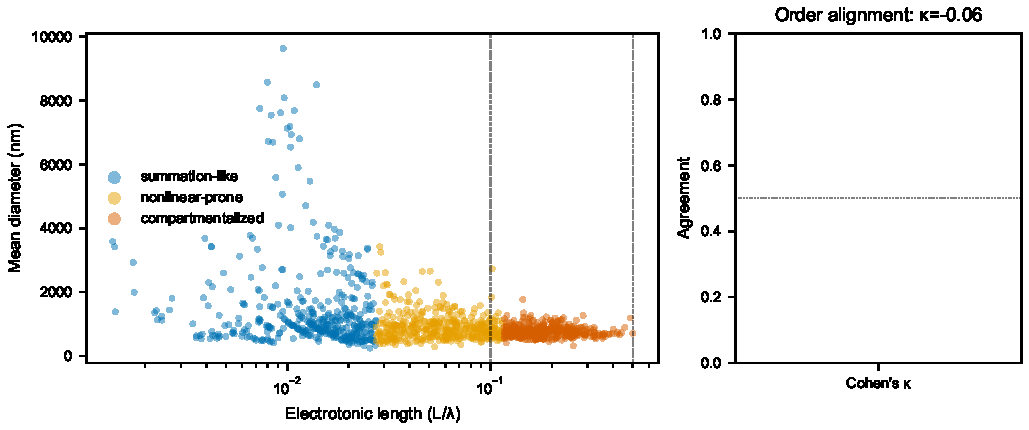
\includegraphics[width=0.85\textwidth]{../figures/fig_regime_classification.pdf}
\caption{Structural regime classification by electrotonic length and diameter. Tertile thresholds on the observed $L/\lambda$ distribution (dashed lines) separate summation-like, nonlinear-prone, and compartmentalized branches. Inset: branch order shows weak correspondence (Cohen's $\kappa = -0.06$), confirming that electrotonic length captures variation beyond topological depth.}
\label{fig:regime}
\end{figure}

\begin{figure}[H]
\centering
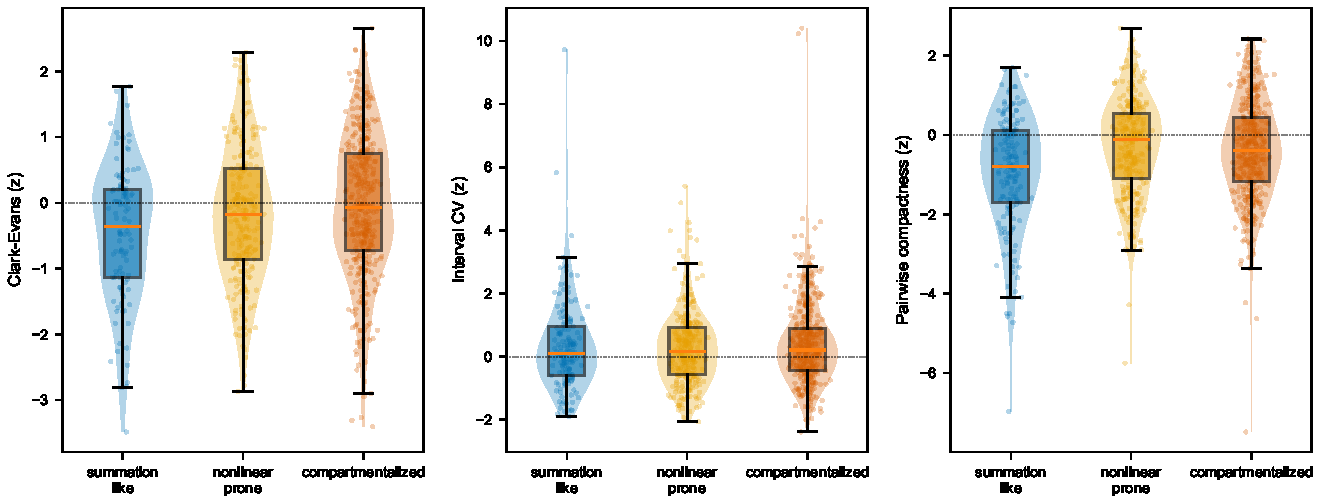
\includegraphics[width=0.95\textwidth]{../figures/fig_spatial_org_by_regime.pdf}
\caption{Spatial organization $z$-scores by structural regime for three independent metrics. Pairwise compactness (left) shows the strongest coupling: summation-like branches are substantially more compact than the geometry-matched null expectation. Clark--Evans (center) trends similarly; interval CV (right) shows no clear regime dependence, indicating the coupling reflects overall clustering rather than spacing regularity.}
\label{fig:coupling}
\end{figure}

\begin{figure}[H]
\centering
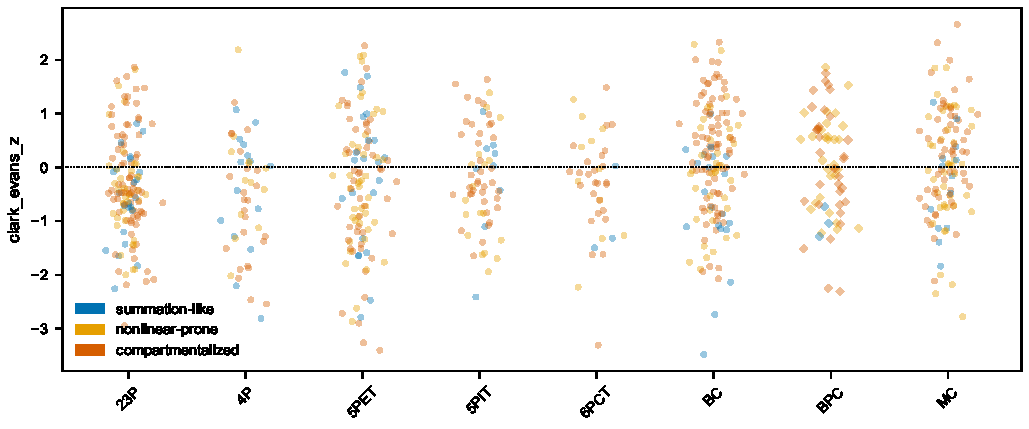
\includegraphics[width=0.95\textwidth]{../figures/fig_cross_cell_type.pdf}
\caption{Cell-type-specific mediation. Excitatory neurons (left) show complete mediation: the direct regime effect vanishes when partner structure is controlled ($c' \approx 0$). Inhibitory neurons (center) show partial mediation: a substantial residual (61\%) persists, indicating a partner-independent organizational axis. Bipolar cells (right) show negligible mediation with minimal partner gradient. Error bars: bootstrap 95\% CI.}
\label{fig:mediation}
\end{figure}

\begin{figure}[H]
\centering
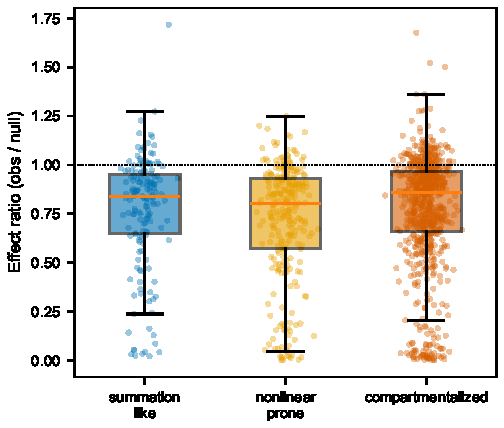
\includegraphics[width=0.8\textwidth]{../figures/fig_partner_compactness.pdf}
\caption{Partner compactness by structural regime. Partners targeting a single regime (non-spanning) show greater compactness (lower effect ratio) than regime-spanning partners. Compactness differs by target regime (Kruskal--Wallis $p = 0.009$).}
\label{fig:partner}
\end{figure}

\begin{figure}[H]
\centering
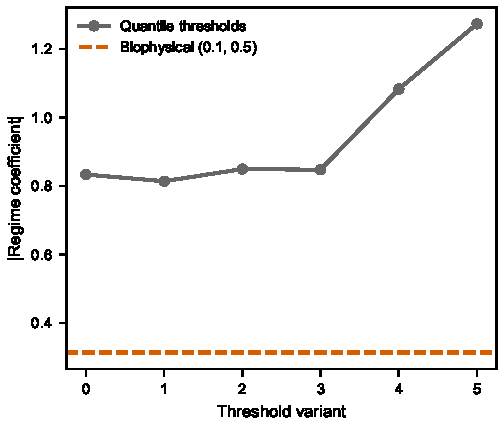
\includegraphics[width=0.8\textwidth]{../figures/fig_sensitivity.pdf}
\caption{Sensitivity analysis: coupling effect size (mixed-model regime coefficient for pairwise compactness $z$-score) across six quantile-based threshold pairs. The primary tertile thresholds are highlighted. Effect size is stable across the threshold range (0.81--1.27), confirming robustness. The biophysical reference thresholds (0.1, 0.5) produce a degenerate split (only 1 compartmentalized branch) and are shown for comparison only.}
\label{fig:sensitivity}
\end{figure}

\clearpage

\section*{Supplementary Figures}

\begin{figure}[H]
\centering
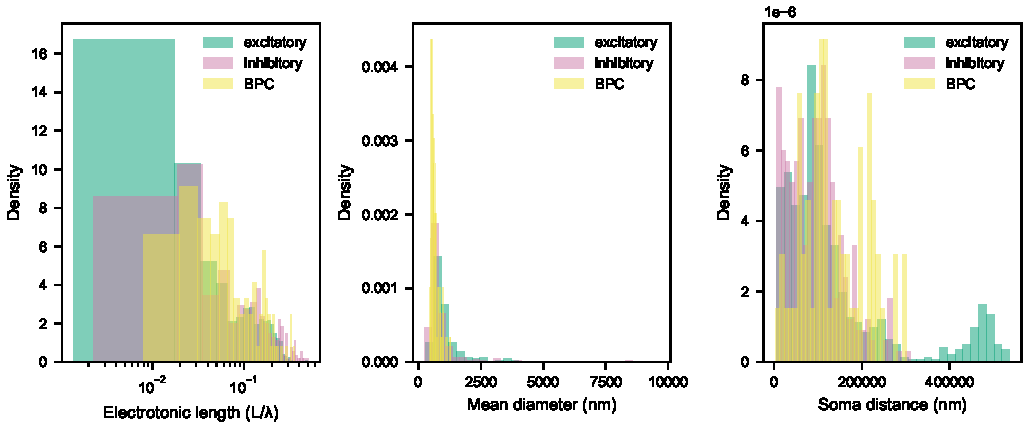
\includegraphics[width=0.9\textwidth]{../figures/fig_branch_morphometry.pdf}
\caption{\textbf{Figure S1.} Distributions of electrotonic length, mean diameter, and soma distance across all 1,234 branches, separated by cell type. The compressed electrotonic length distribution (62\% below $L/\lambda = 0.1$) motivated the use of tertile-based rather than biophysical thresholds for regime classification (Section 2.1). Diameter and soma distance show the expected positive correlation with cell type, with inhibitory neurons tending toward thicker proximal dendrites.}
\label{fig:morphometry}
\end{figure}

\begin{figure}[H]
\centering
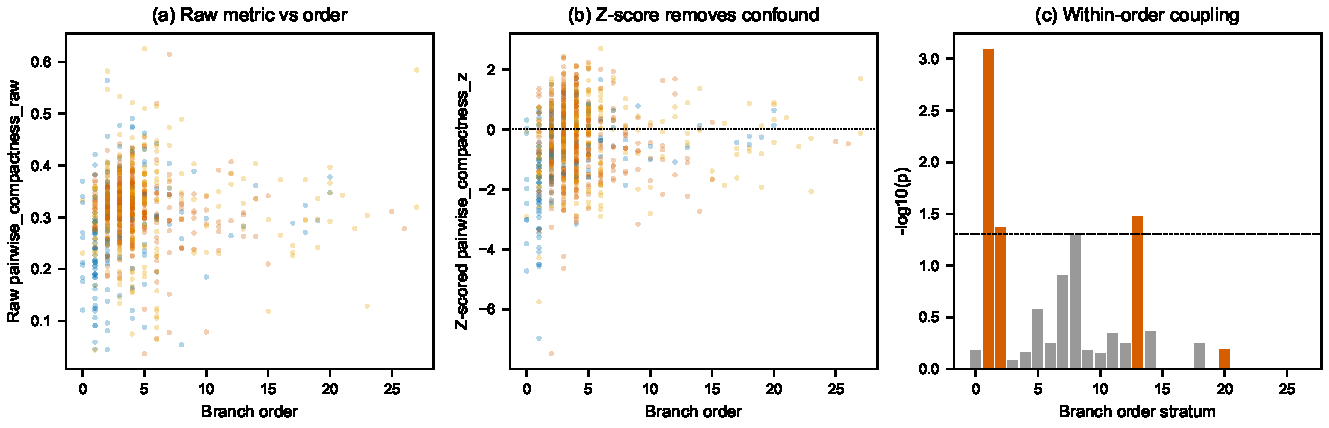
\includegraphics[width=0.8\textwidth]{../figures/fig_confound_control.pdf}
\caption{\textbf{Figure S2.} Confound control details. (a) Raw pairwise compactness versus branch order, showing the expected geometric confound. (b) After $z$-scoring against the per-branch uniform null, the confound is removed. (c) Within-order stratified Kruskal--Wallis: regime coupling persists in the largest strata (order 1: $p = 0.0008$; order 2: $p = 0.043$), confirming the coupling is not an artifact of topological depth. Cited in Section 2.2.}
\label{fig:confound}
\end{figure}

\begin{figure}[H]
\centering
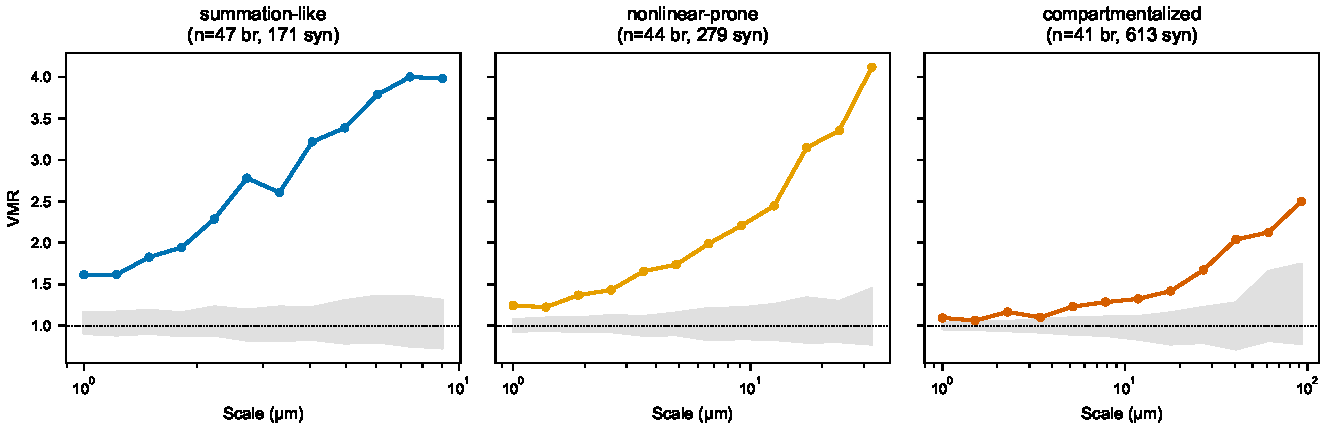
\includegraphics[width=0.8\textwidth]{../figures/fig_regime_grouped_vmr.pdf}
\caption{\textbf{Figure S3.} Variance-mean ratio (VMR) fingerprint curves computed separately for branches in each structural regime, with dendrite-constrained null envelopes (gray). Summation-like branches show elevated VMR at small scales, consistent with the excess clustering detected by pairwise compactness. Compartmentalized branches track closer to the null envelope. This confirms that the branch-level spatial metrics and multiscale VMR analysis yield convergent conclusions about regime-dependent organization (Section 2.2).}
\label{fig:vmr}
\end{figure}

\begin{figure}[H]
\centering
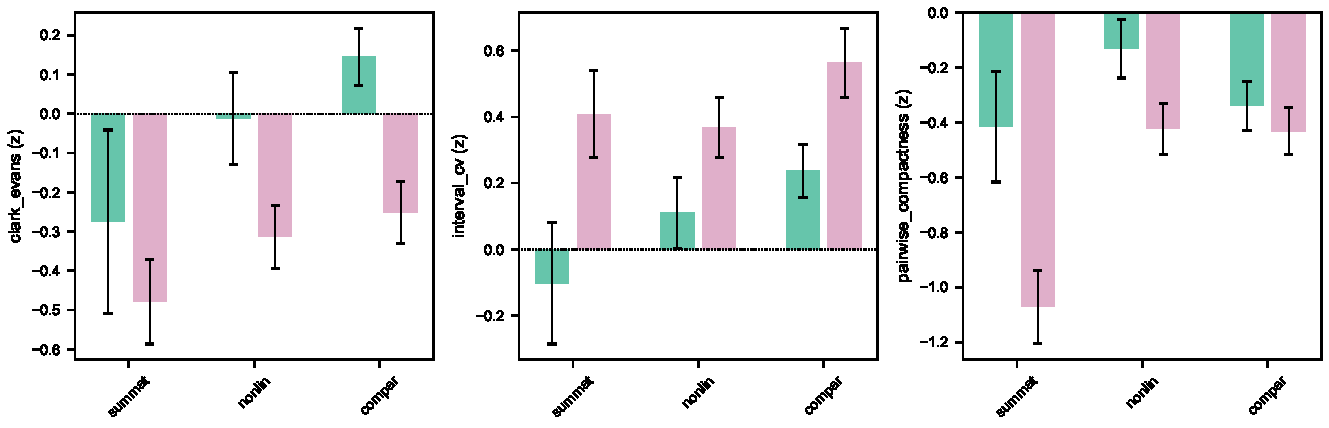
\includegraphics[width=0.8\textwidth]{../figures/fig_input_type_coupling.pdf}
\caption{\textbf{Figure S4.} Excitatory versus inhibitory input spatial organization within each structural regime. Both input types show the same direction of coupling (compact branches more clustered), but excitatory inputs drive a larger fraction of the effect. This is consistent with the complete partner-mediation for excitatory neurons reported in Section 2.4.}
\label{fig:inputtype}
\end{figure}

\bibliographystyle{apalike}
\bibliography{references}

\end{document}
